\Cref{sec:fitting_mbc,sec:background_subtraction} introduced the fitting procedure and \BB background subtraction.
Together with the optimal selections from \Cref{sec:final_optimisation}, this fully defines the analysis strategy from the Belle~II simulated datasets to the \BtoXsgamma spectrum.
However, the defined fitter has to be validated in simulation to give an unbiased estimation of \BtoXsgamma events, with a good resoltion and signal efficiency.
The studies in this Section will show such results.

\subsection{Validation of \texorpdfstring{\Mbc}{Mbc} fit on reduced samble size}\label{sec:mbc_fit_validation_misreconstructed}

The results that were shown in \Cref{fig:mc_fit_yield_comparisons} only provided results for fitting 1.6~\invab -- a dataset about an order of magnitude larger than is expected in the case of this analysis.
Therefore, the generic \MC dataset is pseudorandomly split into 10 smaller subsets, corresponding to 160~\invfb, and each of them are fitted independently.
The choice of 160~\invfb, rather than 190~\invfb which is the sample size of the Belle~II data used in the analysis, is due to anticipated data-simulation differences.
\todo[inline]{see XXX and next paragraph performed where?}
Indeed, a 190~\invfb dataset should correspond to roughly 160~\invfb in simulation due to differences in tag-\B reconstruction efficiency.

The resulting 10 fits and the estimated $\mathcal{N}_{CB}$ corresponding to each \EB bin are shown in \Cref{fig:extracted_validation_mc}.
The expected number of events in each fit is always equal to one tenth of that in the total generic \MC dataset.
It can be observed that all data points, and their average, are statistically compatible with the expectation.
These results indicate, that despite using a 10 times larger dataset to define the \PDF{s}, this \Mbc fit model produces reliable results.
Further tests, particularly a test ensuring that the fitter is unbiased, are performed later.

\begin{figure}[htbp!]
    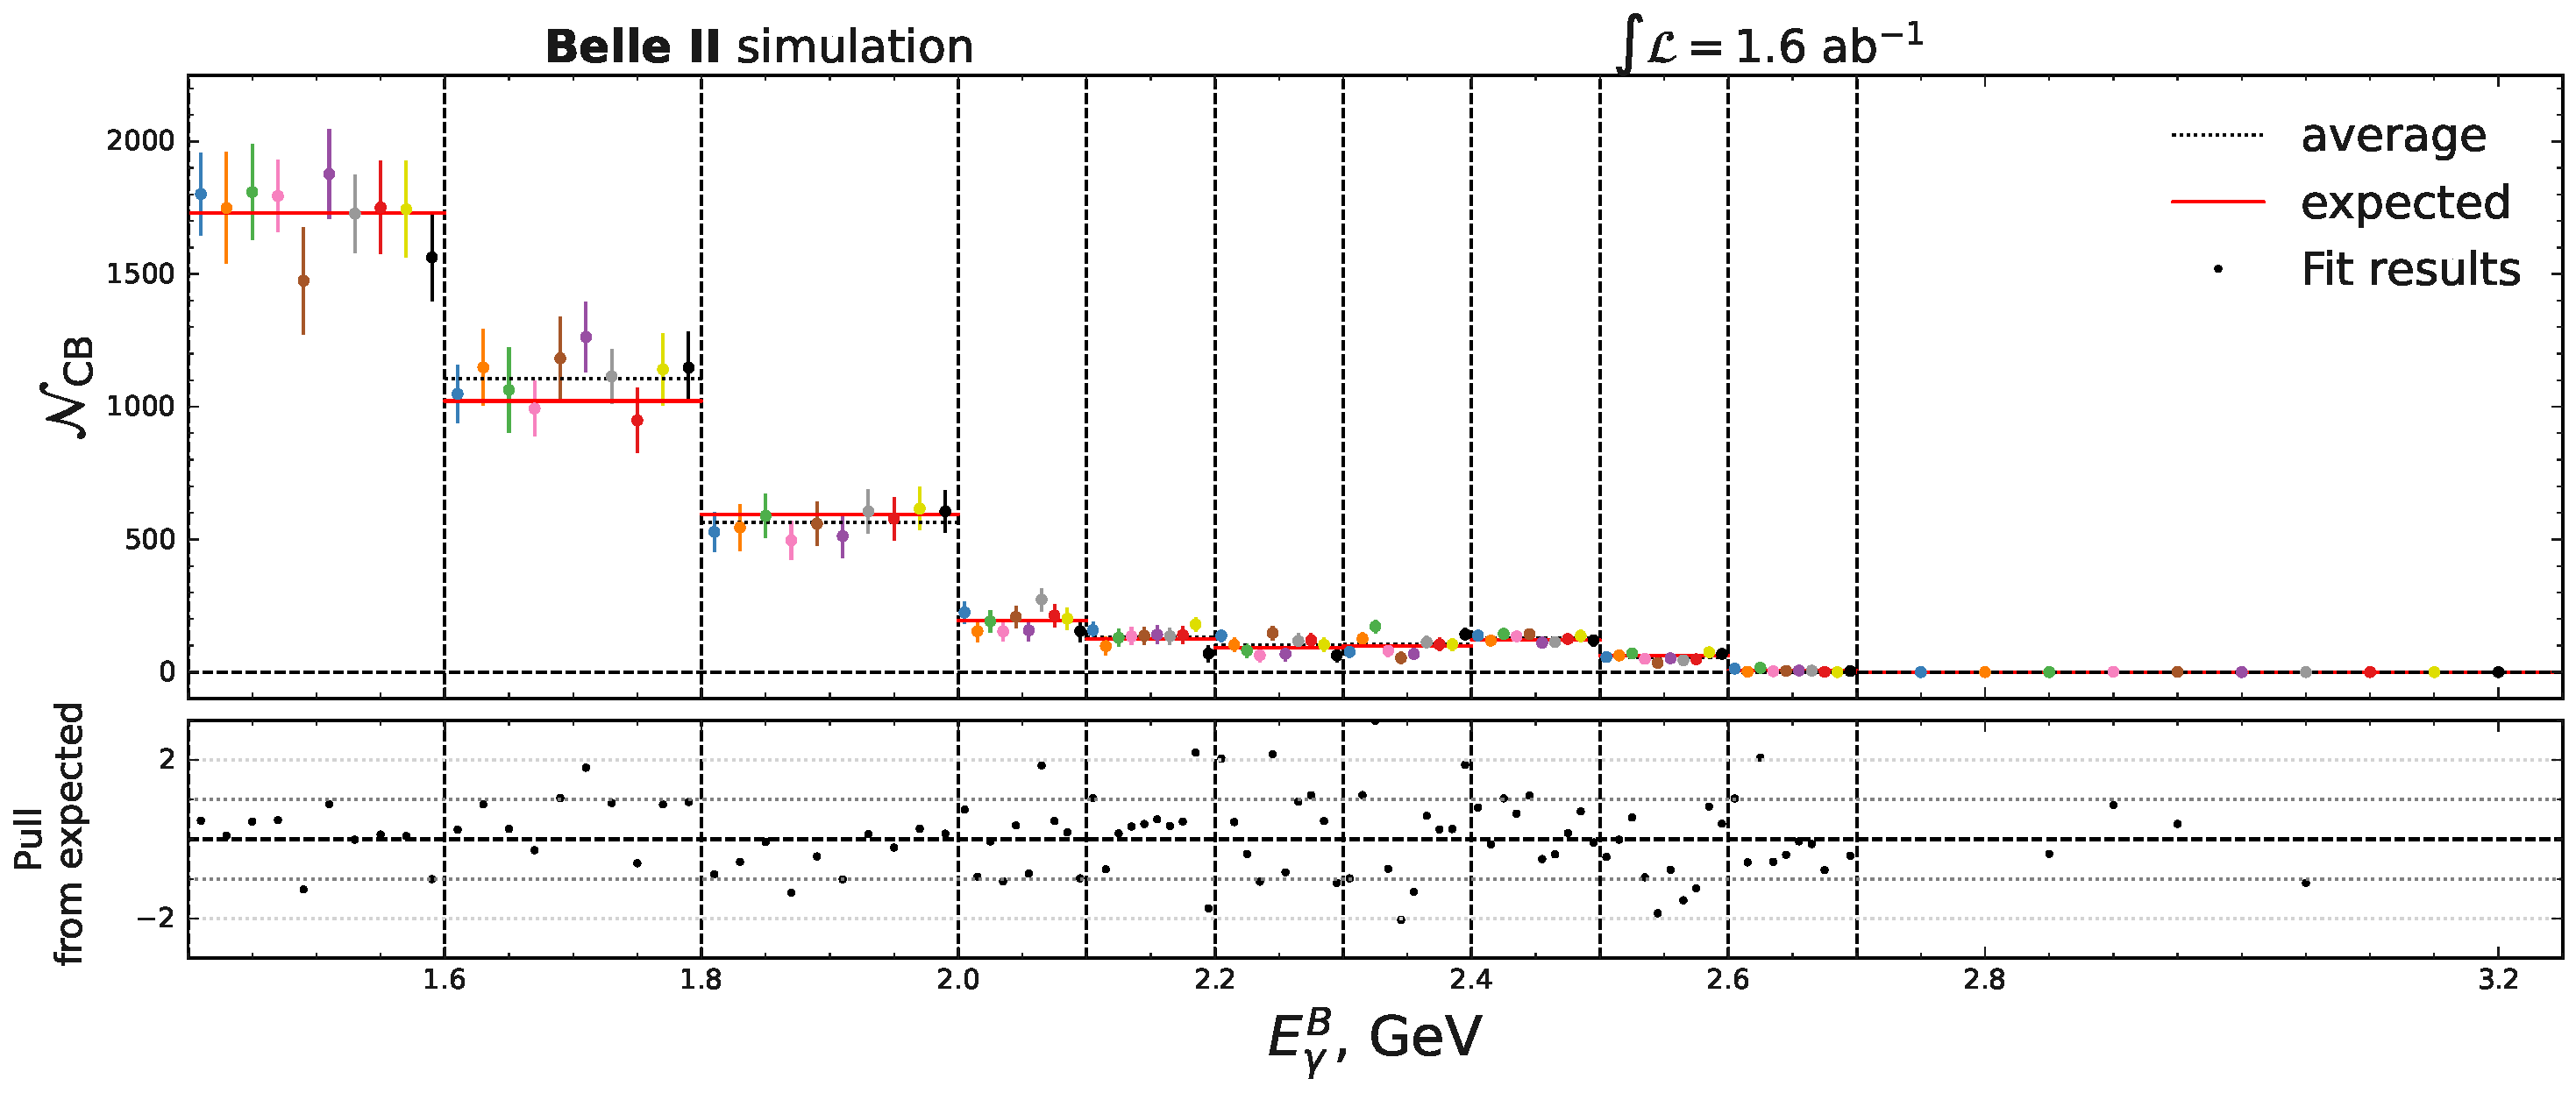
\includegraphics[width=0.9\textwidth]{figures/mc_validation/extracted_signal_generic_mc.pdf}
    \caption{\label{fig:extracted_validation_mc}The estimated $\mathcal{N}_{CB}$ values from fits on one tenth of generic \MC, corresponding to 160~\invfb of simulation.
    The dashed lines represent different \EB bins, each bin showing one data point corresponding to a simultaneous fit of all \EB bins.
    The dotted lines show the average of all 10 points in each bin, whereas the full lines show the number of good tag-\B events in the original 1.6~\invab dataset, scaled down 10 times (`expected').
    The subpanels show the pull of each datapoint from the expected number of events.
    These results show that the fit is able to extract a result on a dataset that is an order of magnitude smaller.
    }
\end{figure}

\subsection{Validation of subtraction of remaining-\texorpdfstring{\BB}{BB} background}\label{sec:background_subtraction_validation_mc}

\begin{figure}[htbp!]
    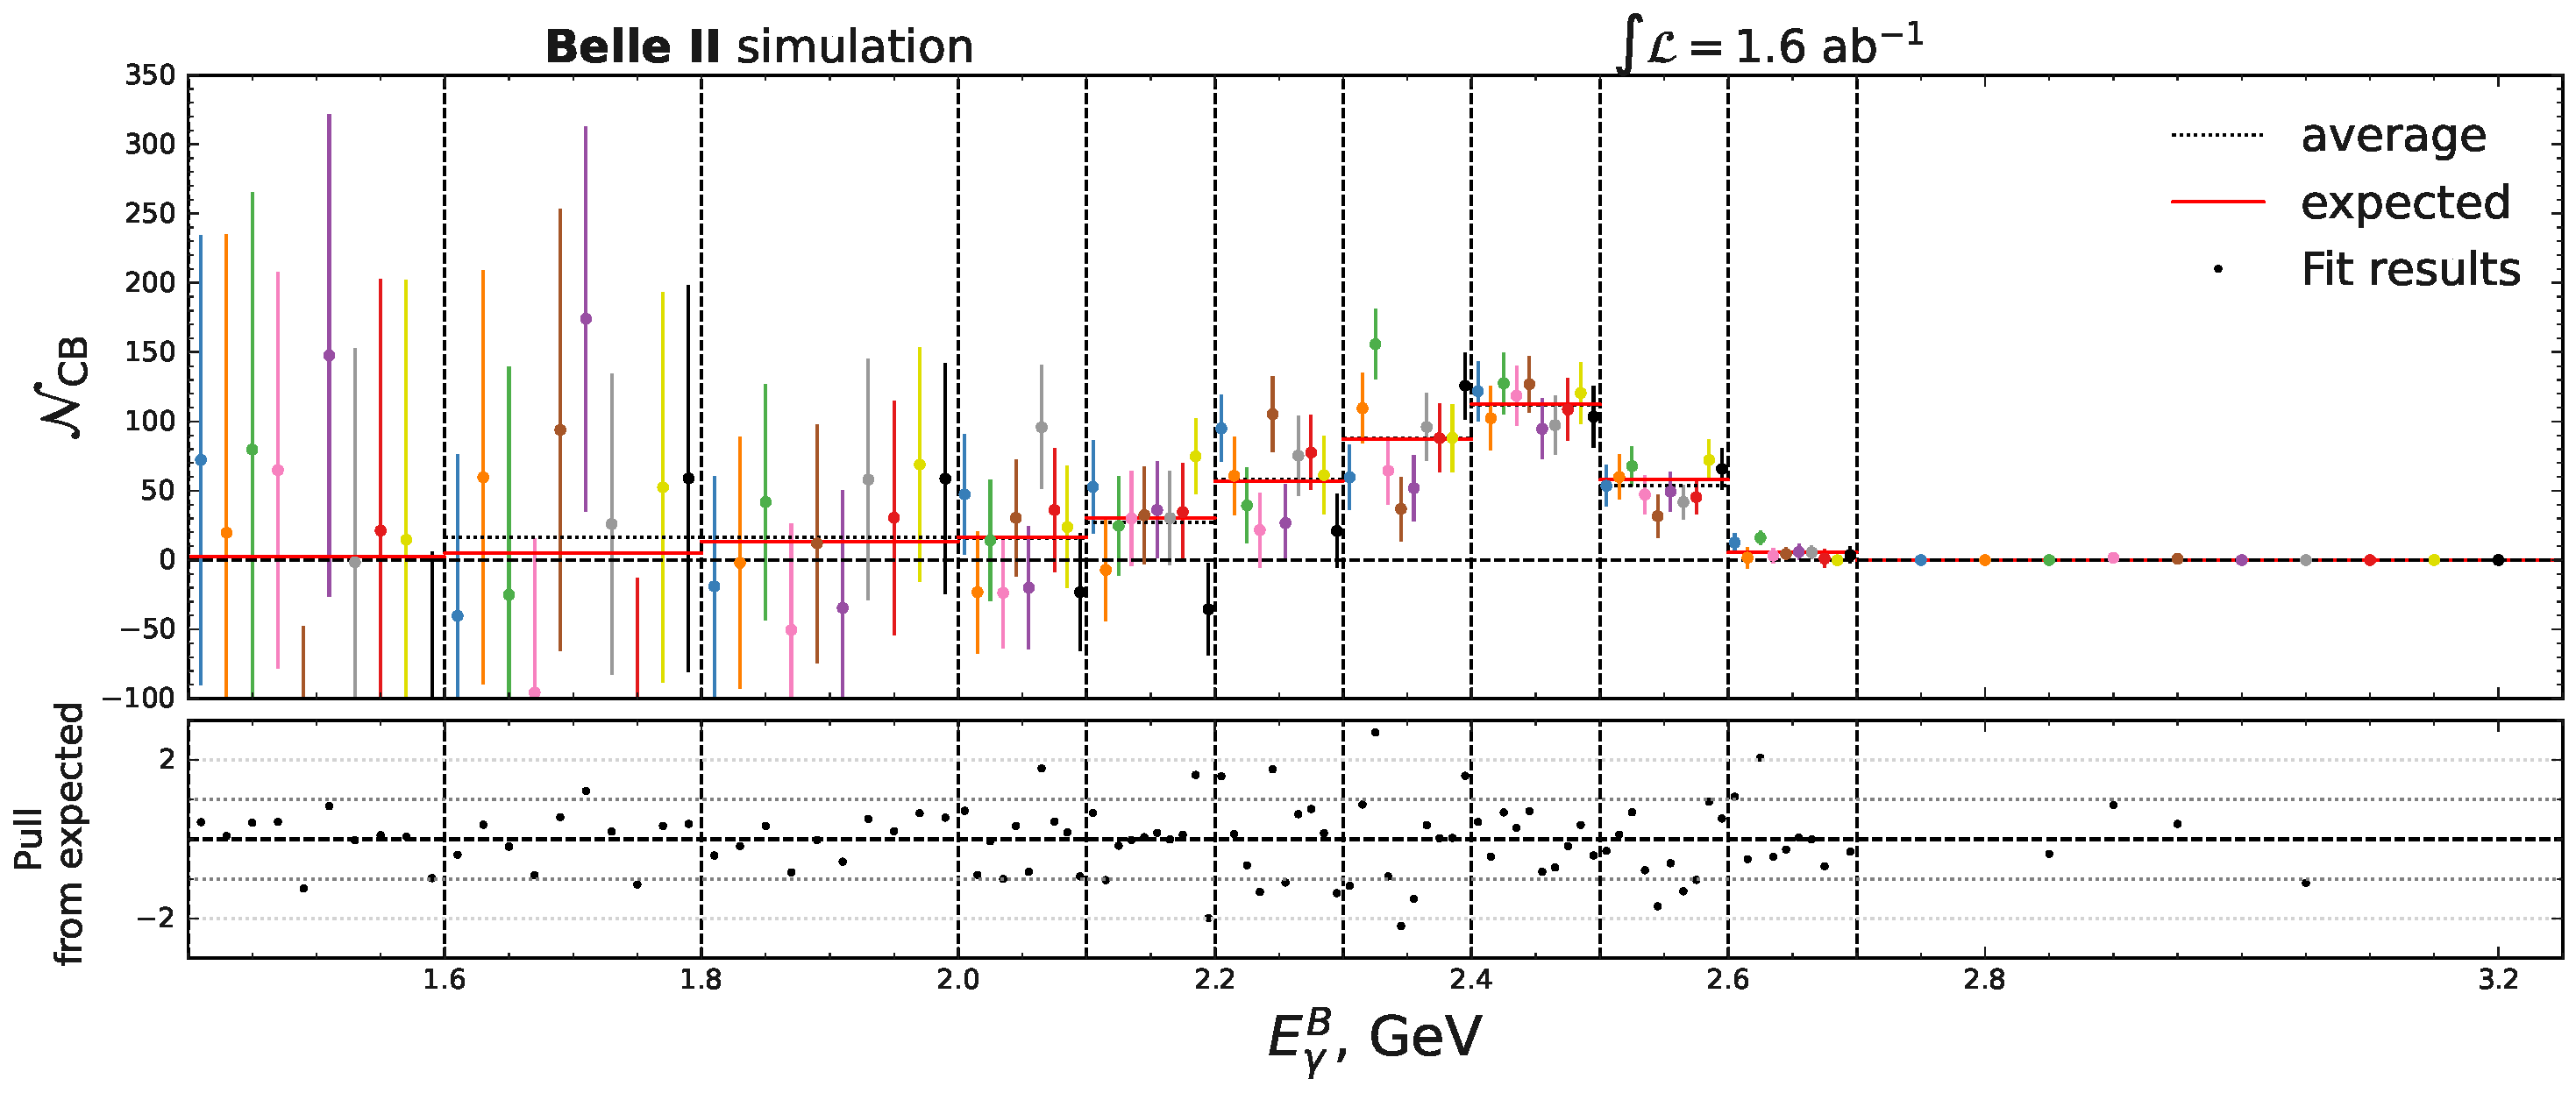
\includegraphics[width=0.9\textwidth]{figures/mc_validation/subtracted_signal_generic_mc.pdf}
    \caption{\label{fig:subtracted_validation_mc}
    The estimated $\mathcal{N}_{CB}$ with subtracted background.
    }
\end{figure}
